\documentclass[10pt,twocolumn]{article}

\usepackage[margin=0.8in,top=0.95in,bottom=0.85in,columnsep=0.3in]{geometry}
\usepackage{mathpazo}
\usepackage{amsmath}
\usepackage{graphicx}
\usepackage{caption}
\usepackage{booktabs}
\usepackage{array}
\usepackage{xcolor}
\usepackage{tikz}
\usetikzlibrary{positioning,arrows.meta,calc}
\usepackage[colorlinks=true,citecolor=blue,linkcolor=blue,urlcolor=blue]{hyperref}
\usepackage[compact]{titlesec}
\usepackage{enumitem}
\usepackage{capt-of}
\usepackage{fancyhdr}
\usepackage{balance}
\clubpenalty=10000
\widowpenalty=10000
\displaywidowpenalty=10000

\setlength{\parindent}{1.1em}
\setlength{\parskip}{0pt}
\setlength{\emergencystretch}{2em}
\captionsetup{font=small,labelfont=bf,labelsep=colon}

\titlespacing*{\section}{0pt}{2.2ex plus .8ex minus .2ex}{1ex}
\titlespacing*{\subsection}{0pt}{1.8ex plus .4ex minus .1ex}{.7ex}
\titleformat{\section}{\normalfont\normalsize\bfseries}{\thesection.}{0.6em}{}
\titleformat{\subsection}{\normalfont\normalsize\bfseries}{\thesubsection.}{0.6em}{}

\pagestyle{fancy}
\fancyhf{}
\renewcommand{\headrulewidth}{0pt}
\fancyhead[C]{\small\itshape A. Gottwein, L. Kemei, J. Chen \& E. Shao / Temporal Anti-Aliasing for Single-Photon Reconstruction}
\fancyfoot[C]{\small\thepage}
\fancypagestyle{plain}{\fancyhf{}\renewcommand{\headrulewidth}{0pt}\fancyfoot[C]{\small\thepage}}

\newcommand{\sref}[1]{Sec.~\ref{#1}}

\begin{document}
\thispagestyle{plain}

\twocolumn[{%
  \hbox to \textwidth{\vtop{\hsize=0.5\textwidth\small\noindent CS 566, Fall 2026\hfil\break Introduction to Computer Vision\hfil\break Prof.\ Mohit Gupta}\hfil\vtop{\hsize=0.5\textwidth\small\raggedleft\itshape Mid-term Report\par October 29, 2026}}
  \vspace{1.6em}
  \begin{center}
    {\Large\bfseries Temporal Anti-Aliasing for Single-Photon Reconstruction}\par\vspace{1.2em}
    {\normalsize Adrian Gottwein \quad Limo Kemei \quad Jack Chen \quad Ethan Shao}\par\vspace{0.15em}
    {\small \texttt{gottwein} \quad \texttt{kkemei} \quad \texttt{zchen843} \quad \texttt{zshao46}}\par\vspace{0.5em}
    {\small University of Wisconsin--Madison}\par\vspace{0.3em}
    {\small Code: \url{https://github.com/1immy/cs566-project} \quad Webpage: \url{https://1immy.github.io/cs566-project/}}
  \end{center}
  \vspace{0.6em}
  \begin{center}
    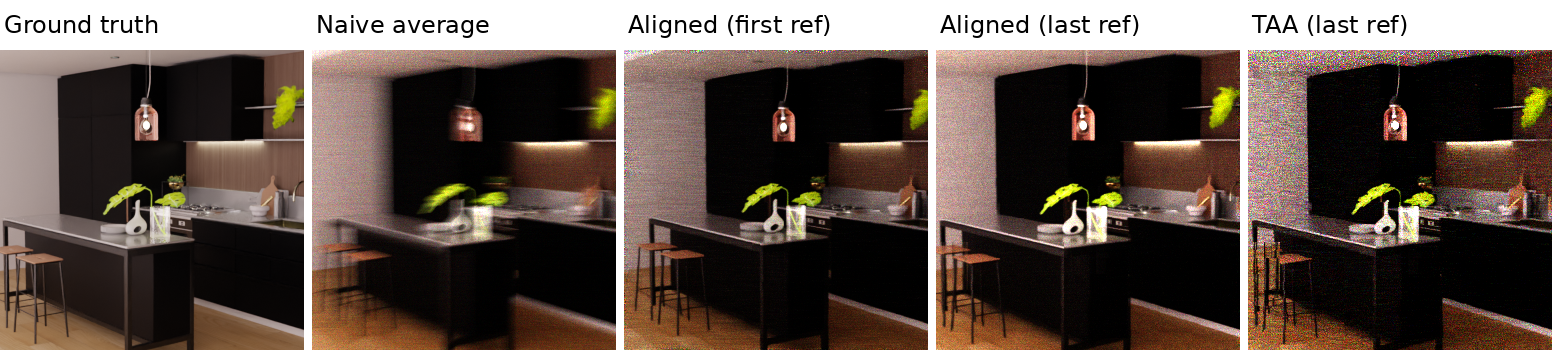
\includegraphics[width=\textwidth]{fig_compare.png}
    \captionof{figure}{Reconstructions of burst 0 of \texttt{kitchen1} (300$\times$304 crop). Naive averaging blurs the moving scene. Aligning to the first group of frames is sharp but offset from the ground truth. Aligning to the last group matches it, with visible photon noise. Default TAA, also with a last-group reference, is noisier still. Each result is scaled by one gain for display.}
    \label{fig:compare}
  \end{center}
  \vspace{0.2em}
  \noindent\rule{\textwidth}{0.4pt}\par\vspace{0.3em}
  \begin{center}
  \begin{minipage}{0.94\textwidth}
  \small\noindent\textbf{Abstract}\par\vspace{0.1em}
  \itshape
  We investigate whether history-validation heuristics from temporal anti-aliasing (TAA), namely neighborhood clamping and motion-adaptive blending, can improve classical align-and-merge reconstruction of single-photon bursts. All stages of our pipeline now run on real Single Photon Challenge data, including an evaluation harness that reports PSNR and SSIM. Two early findings shape the rest of the project. First, the scene moves substantially \emph{inside} a single burst. Second, the ground truth is at the pose of the \emph{last} frames, so the choice of reference frame decides whether alignment helps at all. With the correct reference, block alignment improves on naive averaging by 2.5 to 4.4~dB PSNR on the bursts we tested, while our first TAA configuration is 1 to 4~dB worse than alignment alone. We report these results, the difficulties behind them, and the changes they imply for our plan.
  \end{minipage}
  \end{center}
  \vspace{0.2em}
  \noindent\rule{\textwidth}{0.4pt}
  \vspace{1.2em}
}]

\section{Introduction}

A single-photon camera records a burst of binary frames, each reporting only whether a photon arrived at a pixel during a very short exposure. Averaging many frames recovers brightness, but if the scene or the camera moves during the burst, averaging blurs the result. Aligning the frames before merging removes the blur, at the price of a new failure mode: wrongly aligned content is merged into the output and appears as ghosting.

Real-time rendering faces a closely related problem. Temporal anti-aliasing (TAA) accumulates samples over consecutive frames, reprojects them to compensate for motion, and uses \emph{history validation} to decide how much of the accumulated result to trust~\cite{yang2020survey}. Two validation tools are central: neighborhood clamping, which restricts the history to the color range seen in the current frame~\cite{karis2014}, and adaptive blending, which lowers the weight of history when motion or disagreement is large~\cite{yang2009amortized}. Our project asks whether these tools carry over to single-photon bursts, where the samples are binary and far noisier than in rendering.

This report covers the first half of the project. We describe the pipeline and its current state (\sref{sec:progress}), present the first results on real data (\sref{sec:results}), discuss the difficulties we met (\sref{sec:difficulties}), and list the changes to our proposal and the remaining plan (\sref{sec:changes} and \sref{sec:next}).

\section{Progress}
\label{sec:progress}

\subsection{Pipeline overview}

Figure~\ref{fig:pipeline} shows the pipeline. A loader reads a burst and splits it into groups of consecutive frames, because a single binary frame carries too little signal to align. Each group is averaged and aligned to a reference group. The warped history is then validated against the incoming group and merged, and the result is scored against the ground truth. The four stages follow our fixed interfaces, so each team member can work on one stage independently.

\begin{figure}[t]
\centering
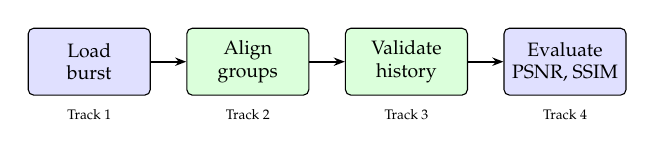
\begin{tikzpicture}[
  box/.style={draw,rounded corners=2pt,minimum height=0.85cm,minimum width=1.55cm,align=center,font=\scriptsize,inner sep=2pt},
  data/.style={box,fill=blue!12},
  proc/.style={box,fill=green!14},
  arr/.style={-{Stealth[length=4pt]},thick}]
  \node[data] (load) {Load\\ burst};
  \node[proc,right=0.45cm of load] (align) {Align\\ groups};
  \node[proc,right=0.45cm of align] (rej) {Validate\\ history};
  \node[data,right=0.45cm of rej] (eval) {Evaluate\\ PSNR, SSIM};
  \draw[arr] (load)--(align);
  \draw[arr] (align)--(rej);
  \draw[arr] (rej)--(eval);
  \node[font=\tiny,below=0.05cm of load] {Track 1};
  \node[font=\tiny,below=0.05cm of align] {Track 2};
  \node[font=\tiny,below=0.05cm of rej] {Track 3};
  \node[font=\tiny,below=0.05cm of eval] {Track 4};
\end{tikzpicture}
\caption{Schematic of the reconstruction pipeline. Green blocks are the components under study, blue blocks are infrastructure.}
\label{fig:pipeline}
\end{figure}

\subsection{Data and infrastructure}

The dataset stores each burst as 1{,}024 binary frames of $800\times800$ RGB, bit-packed along the width. A full burst unpacks to about 2~GB, so our loader supports frame and crop selection directly on the packed array. A 1~MB sample is committed to the repository and a 10-scene slice (about 5~GB) is shared with the team. The full set stays on a private NAS and is used only for final runs. Work is tracked as GitHub issues against course milestones.

\subsection{Alignment}

Each group $g$ is averaged into a frame $\bar{x}_g$. The aligner estimates a motion field by coarse-to-fine $8\times8$ block matching on a three-level pyramid and warps $\bar{x}_g$ to the reference, leaving invalid pixels undefined outside the source. The same aligner is used by every method, so differences between methods are attributable to the merge stage.

\subsection{History validation}

Following the TAA formulation, we maintain a history $h$ with a per-pixel weight $W$ (the number of frame-equivalents it represents, initialized from the first group). Each warped group $\tilde{x}_g$ of $n$ frames is merged as a weighted mean in which the history is discounted by a per-pixel confidence $c\in(0,1]$:
\begin{equation}
  h' = \frac{c\,W\,\hat{h} + n\,\tilde{x}_g}{c\,W + n}, \qquad W' = c\,W + n,
\end{equation}
where $\hat{h}$ is the history clamped, per channel, to the $3\times3$ neighborhood range of $\tilde{x}_g$ widened by a margin of 0.05. The confidence falls with the disagreement $\delta=\max_k|h_k-\hat{h}_k|$ (how far the history lies outside that range) and with the displacement $d$ in pixels reported by the aligner:
\begin{equation}
  c = \frac{\exp(-\delta/0.1)}{1 + d/8}.
\end{equation}
Pixels with no valid observation keep their history and weight unchanged. Component switches recover the aligned baseline exactly, and synthetic experiments showed both helpful and harmful rejection regimes, which motivated testing on real data.

\subsection{Evaluation}

The evaluation module provides an \texttt{evaluate} function that returns the mean per-channel PSNR and SSIM (7$\times$7 uniform window, reflect padding). A harness runs naive averaging, aligned averaging and TAA on a set of bursts, accepts additional pipelines as plug-ins, and writes a results table and comparison figures. It applies one fixed intensity rule to every method, $\mathrm{clip}(2.7\,x,0,1)$, where the gain of 2.7 is a placeholder that is not calibrated to the camera response. The full suite of 48 unit tests passes.

\section{Current Results}
\label{sec:results}

\subsection{Setup}

Table~\ref{tab:psnr} uses scene \texttt{kitchen1}, bursts 0, 1 and 10, a $300\times304$ central crop, all 1{,}024 frames, in groups of 64. The ground truth is much brighter than the photon average, with a least-squares gain of about 3 to 4 on these crops. For this table we therefore multiply each reconstruction $\hat{y}$ by a single per-image gain $g^\star$ before computing PSNR:
\begin{equation}
  g^\star = \frac{\langle \hat{y}, y\rangle}{\langle \hat{y}, \hat{y}\rangle}.
\end{equation}
This differs from the harness, which uses the fixed gain above, and the two rules are not yet unified (\sref{sec:difficulties}). The results come from one scene and no held-out data, so they are indicative, not a benchmark.

\subsection{Motion inside a burst}

Phase correlation between 256-frame windows shows a mostly horizontal drift from the first to the last window of about 9, 20 and 2~px for the three bursts. The offset between the ground truth and the first window is 13, 25 and 2~px along $x$, and it falls to about 1~px or less at the last window. The ground truth is therefore the pose at the end of the burst, not the start.

\subsection{Reconstruction quality}

Table~\ref{tab:psnr} lists the PSNR of each method. Aligning to the last group beats naive averaging by 2.5 to 4.4~dB. The fixed first-group reference used in our first runs is 2.2 to 2.9~dB \emph{worse} than naive averaging, because it moves the output away from the ground-truth pose. The clamp alone is inert on two bursts at its default margin and costs 0.6~dB on the third. The full TAA configuration loses 1.0 to 3.8~dB against plain alignment, most on the fastest burst.

\begin{table}[t]
\centering
\small
\renewcommand{\arraystretch}{1.0}
\begin{tabular}{@{}p{0.5\columnwidth}ccc@{}}
\toprule
\textbf{PSNR (dB)} & \textbf{b0} & \textbf{b1} & \textbf{b10} \\
\midrule
Naive average & 16.2 & 14.7 & 16.8 \\
Aligned, first-group ref. & 14.0 & 12.5 & 13.9 \\
Aligned, last-group ref. & \textbf{19.7} & \textbf{19.1} & \textbf{19.3} \\
Clamp only, last-group ref. & 19.7 & 18.5 & 19.3 \\
TAA (default), last-group ref. & 17.3 & 15.3 & 18.3 \\
\bottomrule
\end{tabular}
\caption{Per-image gain-matched PSNR on \texttt{kitchen1}, bursts 0, 1 and 10, full bursts. Last-group reference results come from running the same code on the time-reversed burst.}
\label{tab:psnr}
\end{table}

\subsection{Evaluation harness}

Table~\ref{tab:harness} shows the harness output on the two committed samples, which use 256 frames and a $128\times128$ crop, the fixed gain of 2.7, and the first-group reference. Aligned averaging and TAA do not beat naive averaging here on either metric, and TAA is essentially equal to alignment in PSNR and slightly lower in SSIM. This agrees with the first-group result in Table~\ref{tab:psnr}. The absolute values are low (PSNR below 12~dB, SSIM below 0.16) because the fixed gain and the pose offset both penalize every method. These numbers are not comparable with Table~\ref{tab:psnr}: the crop, the number of frames, the reference group and the intensity rule all differ.

\begin{table}[t]
\centering
\small
\begin{tabular}{@{}lcccc@{}}
\toprule
 & \multicolumn{2}{c}{\textbf{Burst 0}} & \multicolumn{2}{c}{\textbf{Burst 1}} \\
\cmidrule(lr){2-3}\cmidrule(lr){4-5}
 & PSNR & SSIM & PSNR & SSIM \\
\midrule
Naive average & 11.93 & 0.159 & 9.78 & 0.140 \\
Aligned (first ref.) & 11.86 & 0.150 & 9.52 & 0.134 \\
TAA (first ref.) & 11.86 & 0.148 & 9.52 & 0.128 \\
\bottomrule
\end{tabular}
\caption{Harness output on the committed samples (256 frames, $128\times128$ crop, fixed gain 2.7, first-group reference). PSNR in dB.}
\label{tab:harness}
\end{table}

\section{Difficulties}
\label{sec:difficulties}

\paragraph{Reference frame.}
The ground-truth pose is the end of the burst. A fixed first-group reference, the natural default, makes alignment look harmful. We found this only after comparing against the ground truth at several time offsets.

\paragraph{Intensity mismatch.}
Photon averages and the ground-truth image differ in brightness response, so raw PSNR is misleading. We currently use two rules: a per-image least-squares gain for Table~\ref{tab:psnr} and a fixed gain of 2.7 in the harness. One rule must be applied to every method and scene, and this decision is still open.

\paragraph{Noise versus motion.}
Single binary frames cannot be aligned, so we align 64-frame groups. Photon noise in flat regions still produces apparent motion, which makes displacement an unreliable proxy for alignment error.

\paragraph{TAA tuning.}
Our confidence term lowers the history weight with displacement. Once alignment has compensated for the motion, this discards correct frames and raises noise.

\paragraph{Data format and memory.}
Bursts are bit-packed and a full cube unpacks to about 2~GB, so we load by frame and crop and the team works from samples and a shared slice.

\section{Changes to the Proposal}
\label{sec:changes}

\begin{itemize}[leftmargin=1.2em,itemsep=2pt,topsep=3pt]
  \item \textbf{Alignment unit.} Alignment runs within a burst, on groups of frames, with the last group as reference.
  \item \textbf{Motion sweeps.} Real bursts already span roughly 2 to 20~px of motion, so the \texttt{visionsim} sweeps become optional and the motion study uses real bursts binned by measured speed.
  \item \textbf{Data size.} The average archive is about 2.7~GB (133~GB compressed in total), not 8.5~GB as proposed. We use a 10-scene shared slice and run final experiments on the full set.
  \item \textbf{Hypothesis.} The initial TAA result is negative: when alignment is accurate, displacement-based rejection hurts. We now plan a confidence based on alignment residual, and we will report the failure analysis either way.
\end{itemize}

\section{Next Steps}
\label{sec:next}

We will unify the intensity rule, switch the baselines and TAA to the last-group reference, and rerun the harness on full bursts and a motion-binned scene set. We will replace the displacement term with a residual-based confidence and run ablations (clamp, blend, confidence) together with a failure analysis against motion speed. Experiments freeze on Nov.~30. The final presentation is on Dec.~8 and the project webpage is due Dec.~10.

\begin{thebibliography}{9}\small
\bibitem{yang2020survey} L.~Yang, S.~Liu, M.~Salvi. A survey of temporal antialiasing techniques. \emph{Computer Graphics Forum}, 39(2), 2020.
\bibitem{yang2009amortized} L.~Yang, D.~Nehab, P.~V.~Sander, P.~Sitthi-amorn, J.~Lawrence, H.~Hoppe. Amortized supersampling. \emph{ACM Trans.\ Graphics}, 28(5), 2009.
\bibitem{karis2014} B.~Karis. High-quality temporal supersampling. SIGGRAPH Advances in Real-Time Rendering course, 2014.
\end{thebibliography}

\balance
\end{document}
